\chapter{Experiments}
\label{ch:appendix-experiments}

In this appendix, we provide experimental results complementing the
discussion in Chapter \ref{ch:experiments}. 

\section{Evaluation}
\label{sec:appendix-experiments-evaluation}

We claimed that the negative log-likelihood is unsuited for evaluation
partly because it favors ``unsure'' predictions, \ie occupancy probabilities
close to $0.5$ over very certain predictions with few mistakes. The following
example is intended to illustrate this:

\begin{example}
  We consider a $R$-dimensional binary volume representing a shape. Let 
  $y \in [0,1]^R$ the predicted shape; let $y^* \in \{0,1\}^R$ be the true shape.
  Assuming $y$ fits $y^*$ perfectly, the negative log-likelihood is zero.
  Flipping the prediction of one $y_i = 1$ to $y_i \approx 0.0001$ (due to
  numerical stability) changes the negative log likelihood to $\sim 9.21$.
  Then, we can set
  $\frac{-\ln 0.0001}{- \ln 0.5} \approx \frac{9.21}{0.693} \approx 9.966$
  of $y^*$'s occupied voxels to $0.5$ and the negative log-likelihood will not exceed $9.21$.
  In practice, this means that an ``unsure'' model predicting an occupancy probability
  of $0.5$ for many pixels will have a lower negative log-likelihood
  than a nearly perfect prediction with few but very certain mistakes.
\end{example}

\section{2D Example}
\label{sec:appendix-experiments-2d}

\subsection{Shape Prior}

\begin{figure}
  \centering
  \begin{subfigure}[t]{0.48\textwidth}
    \begin{tikzpicture}
      \begin{axis}[
          % https://tex.stackexchange.com/questions/68577/compiling-a-document-with-pgfplots-processing-only-every-x-th-data-point
          each nth point=2,
          filter discard warning=false,
          unbounded coords=discard,
          % https://tex.stackexchange.com/questions/13816/dimension-too-large-while-plotting-with-pgfplots
          %restrict y to domain=0:0.1,
          %restrict x to domain=0:250000,
          ymin=0,
          ymax=0.08,
          xmin=0,
          xmax=250000,
          %xticklabel={
          %  \pgfmathparse{\tick/1000}
          %  \pgfmathprintnumber{\pgfmathresult}k
          %},
          xtick={0,50000,100000,150000,200000,250000},
          xticklabels={0,50k,100k,150k,200k,250k},
          xticklabel style={
            /pgf/number format/fixed
          },
          scaled x ticks=false,
          yticklabel style={
            /pgf/number format/fixed
          },
          scaled y ticks=false,
          %x coord trafo/.code={\pgfmathparse{\pgfmathresult/1000}},
          %xticklabel=\pgfmathprintnumber{\tick}k,
          width=7.5cm,
          height=5cm,
          % https://tex.stackexchange.com/questions/48620/pgfplots-alignment-and-size-of-math-in-legend
          legend cell align=left,
        ]
        
        % https://tex.stackexchange.com/questions/276869/reading-an-unusual-coordinates-file-in-pgfplots
        \addplot +[mark=none] table[ignore chars={(,)},col sep=comma] {data/experiments/2d/vae_occ/easy_5/training_bce.txt};
        \addlegendentry{$\mathcal{L}_{\text{BCE}}$ (train)};
        \addplot +[mark=none] table[ignore chars={(,)},col sep=comma] {data/experiments/2d/vae_occ/easy_5/training_kld.txt};
        \addlegendentry{$\KL$ (train)};
        \addplot +[mark=none] table[ignore chars={(,)},col sep=comma] {data/experiments/2d/vae_occ/easy_5/training_abs.txt};
        \addlegendentry{$\Abs$ (train)};
        
        \addplot +[mark=none] table[ignore chars={(,)},col sep=comma] {data/experiments/2d/vae_occ/easy_5/validation_bce.txt};
        \addlegendentry{$\mathcal{L}_{\text{BCE}}$ (val)};
        \addplot +[mark=none] table[ignore chars={(,)},col sep=comma] {data/experiments/2d/vae_occ/easy_5/validation_kld.txt};
        \addlegendentry{$\KL$ (val)};
        \addplot +[mark=none] table[ignore chars={(,)},col sep=comma] {data/experiments/2d/vae_occ/easy_5/validation_abs.txt};
        \addlegendentry{$\Abs$ (val)};
      \end{axis}
    \end{tikzpicture}
  \end{subfigure}\hfill
  \begin{subfigure}[t]{0.48\textwidth}
    \begin{tikzpicture}
      \begin{axis}[
          % https://tex.stackexchange.com/questions/68577/compiling-a-document-with-pgfplots-processing-only-every-x-th-data-point
          each nth point=2,
          filter discard warning=false,
          unbounded coords=discard,
          % https://tex.stackexchange.com/questions/13816/dimension-too-large-while-plotting-with-pgfplots
          %restrict y to domain=0:0.1,
          %restrict x to domain=0:250000,
          ymin=0,
          ymax=0.08,
          xmin=0,
          xmax=250000,
          %xticklabel={
          %  \pgfmathparse{\tick/1000}
          %  \pgfmathprintnumber{\pgfmathresult}k
          %},
          xtick={0,50000,100000,150000,200000,250000},
          xticklabels={0,50k,100k,150k,200k,250k},
          xticklabel style={
            /pgf/number format/fixed
          },
          scaled x ticks=false,
          yticklabel style={
            /pgf/number format/fixed
          },
          scaled y ticks=false,
          %x coord trafo/.code={\pgfmathparse{\pgfmathresult/1000}},
          %xticklabel=\pgfmathprintnumber{\tick}k,
          width=7.5cm,
          height=5cm,
          % https://tex.stackexchange.com/questions/48620/pgfplots-alignment-and-size-of-math-in-legend
          legend cell align=left,
        ]
        
        \addplot +[mark=none] table[ignore chars={(,)},col sep=comma] {data/experiments/2d/vae_occ/easy_25/training_bce.txt};
        \addlegendentry{$\mathcal{L}_{\text{BCE}}$ (train)};
        \addplot +[mark=none] table[ignore chars={(,)},col sep=comma] {data/experiments/2d/vae_occ/easy_25/training_kld.txt};
        \addlegendentry{$\KL$ (train)};
        \addplot +[mark=none] table[ignore chars={(,)},col sep=comma] {data/experiments/2d/vae_occ/easy_25/training_abs.txt};
        \addlegendentry{$\Abs$ (train)};
        
        \addplot +[mark=none] table[ignore chars={(,)},col sep=comma] {data/experiments/2d/vae_occ/easy_25/validation_bce.txt};
        \addlegendentry{$\mathcal{L}_{\text{BCE}}$ (val)};
        \addplot +[mark=none] table[ignore chars={(,)},col sep=comma] {data/experiments/2d/vae_occ/easy_25/validation_kld.txt};
        \addlegendentry{$\KL$ (val)};
        \addplot +[mark=none] table[ignore chars={(,)},col sep=comma] {data/experiments/2d/vae_occ/easy_25/validation_abs.txt};
        \addlegendentry{$\Abs$ (val)};
      \end{axis}
    \end{tikzpicture}
  \end{subfigure}
  % TODO short caption
  \caption{Binary cross entropy loss $\mathcal{L}_{\text{BCE}}$
  and the Kullback-Leibler divergence $\KL$ on training and validation set for
  the two \VAEs trained in Figure \ref{fig:experiments-2d-vae-occ-5},
  \ie for $Q = 5$ (left) and $Q = 25$ (right).}
  \label{fig:appendix-experiments-2d-vae-occ-5}
\end{figure}

For all experiments regarding occupancy, we used an initial learning rate 
of $\gamma^{(0)} = 5\cdot 10^{-6}$ with $\alpha_{\gamma} = 0.95$,
$\alpha_{\min} = 10^{-12}$ and $T_{\gamma} = 500$. Additionally, a momentum
term of $\beta^{(0)} = 0.5$ with $\alpha_{\beta} = 1.025$,
$\beta_{\max} = 0.9$ and $T_{\beta} = 500$ was used. Optimization
was performed using stochastic gradient descent with batch size of $B = 16$ and
weight decay as regularizer with weight $\kappa = 10^{-6}$; although
we did not find weight decay to have a significant impact. Weights are initialized
using Xavier's approach with. The comparably low
batch size of $16$ is motivated by the fact that the batch size is naturally
limited by the GPU memory in the 3D examples; we wanted to use the same batch size
across 2D and 3D datasets for comparison. The reported results represent the 
early stopping model, \ie the model exhibiting the lowest loss (reconstruction
loss plus Kullback-Leibler divergence). However, we found that early stopping did
not have a significant impact due to the large size of the training set
($10000$ samples for training; $1000$ samples for validation).
For learning signed distance functions (as well as both occupancy and
signed distance functions), we use the same training setup but decrease
the initial learning rate to $\gamma^{(0)} = 5\cdot 10^{-8}$.

\begin{figure}
  \centering
  % http://pgfplots.sourceforge.net/gallery.html
  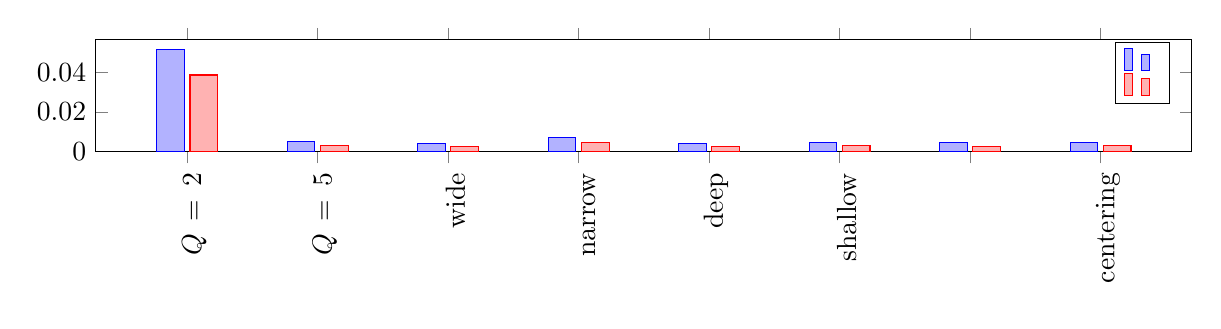
\begin{tikzpicture}
    \begin{axis}[
        ybar,
        % https://tex.stackexchange.com/questions/119887/remove-the-scientific-notation-which-is-unreasonable
        yticklabel style={
          /pgf/number format/fixed,
          /pgf/number format/precision=5
        },
        scaled y ticks=false,
        %legend style={
        %  at={(1.05,1)},
        %  anchor=north west,
        %},
        % https://tex.stackexchange.com/questions/48620/pgfplots-alignment-and-size-of-math-in-legend
        legend cell align=left,
        % https://tex.stackexchange.com/questions/135595/how-to-correct-problem-with-ybar-plot-bad-axis-and-too-many-labels-in-x-axis
        xtick={
          1, 2, 3, 4,
          5, 6, 7, 8
        },
        xticklabels={
          \VAE\\$Q = 2$, \VAE\\$Q = 5$,
          \VAE\\wide, \VAE\\narrow, \VAE\\deep, \VAE\\shallow,
          \DVAE, \VAE\\centering
        },
        x tick label style={text width=1.5cm,align=right},
        ymin=0,
        height=3cm,
        width=15.5cm,
        % https://tex.stackexchange.com/questions/271027/pgfplots-how-to-rotate-extra-x-tick-labels
        x tick label style={
          rotate=90,
          anchor=east,
        },
      ]
        
      % Abs
      \addplot coordinates {
        (1, 0.05121126)
        (2, 0.00515391)
        (3, 0.00391921)
        (4, 0.00682976)
        (5, 0.00391012)
        (6, 0.00462826)
        (7, 0.00437365)
        (8, 0.00459435)
      };
      \addlegendentry{\Abs}
      % AbsThr
      \addplot coordinates {
        (1, 0.03853159)
        (2, 0.00318352)
        (3, 0.00245013)
        (4, 0.00437225)
        (5, 0.00242784)
        (6, 0.00289965)
        (7, 0.00264389)
        (8, 0.00277662)
      };
      \addlegendentry{\AbsThr}
    \end{axis}
  \end{tikzpicture}
  % TODO short caption
  \caption{Absolute error \Abs and its thresholded pendant \AbsThr \VAE considering
  different architecture changes and training procedures. As also detailed in the text,
  a wider architecture with double the number of channels as well as shallow architecture
  with half the number of channels was trained; additionally a shallow variant with
  3 stages of convolutional layers and a deep variant with 5 stages of convolutional
  layers was tested. Finally, we also trained a denoising variational auto-enocder, \DVAE,
  and experimented with centering the training data.}
  \label{fig:appendix-experiments-architecture}
\end{figure}

In Figure \ref{fig:appendix-experiments-architecture}, we experimented
with two approaches to improve training as well as the learned latent space:
centering the training data (by its mean) as well as adding random
salt-and-pepper noise, \ie training a denoising variational auto-encoder (\DVAE).
We also experimented with different architectural changes. In particular,
we experimented with a wider as well as a narrower architecture, meaning that
the number of channels in each layers was doubled of halved. Similarly, we trained
an architecture with five stages of convolutional layers (deep) and the
shallow pendant with only three stages of convolutional layers. The incluence
of all these changes were, however, insignificant. Of course, more weights
(as \ie in the wider and deeper architectures) leads to a lower reconstruction
loss; similarly centering speeds up training and noisy inputs reduces
reconstruction error. However, these gains are negligible and do usually not
influence the learned latent space.

\begin{figure}
  \centering
  \begin{subfigure}[t]{0.48\textwidth}
    \begin{tikzpicture}
      \begin{axis}[
          % https://tex.stackexchange.com/questions/68577/compiling-a-document-with-pgfplots-processing-only-every-x-th-data-point
          each nth point=4,
          filter discard warning=false,
          unbounded coords=discard,
          % https://tex.stackexchange.com/questions/13816/dimension-too-large-while-plotting-with-pgfplots
          %restrict y to domain=0:0.1,
          %restrict x to domain=0:250000,
          ymin=0,
          ymax=0.2,
          xmin=0,
          xmax=500000,
          %xticklabel={
          %  \pgfmathparse{\tick/1000}
          %  \pgfmathprintnumber{\pgfmathresult}k
          %},
          xtick={0,100000,250000,500000},
          xticklabels={0,100k,250k,500k},
          xticklabel style={
            /pgf/number format/fixed
          },
          scaled x ticks=false,
          yticklabel style={
            /pgf/number format/fixed
          },
          scaled y ticks=false,
          %x coord trafo/.code={\pgfmathparse{\pgfmathresult/1000}},
          %xticklabel=\pgfmathprintnumber{\tick}k,
          width=7.5cm,
          height=5cm,
          % https://tex.stackexchange.com/questions/48620/pgfplots-alignment-and-size-of-math-in-legend
          legend cell align=left,
        ]
        
        \addplot +[mark=none] table[ignore chars={(,)},col sep=comma] {data/experiments/2d/vae_sdf/easy_5_long/training_bce.txt};
        \addlegendentry{$\mathcal{L}_{\text{BCE}}$ (train)};
        \addplot +[mark=none] table[ignore chars={(,)},col sep=comma] {data/experiments/2d/vae_sdf/easy_5_long/training_kld.txt};
        \addlegendentry{$\KL$ (train)};
        \addplot +[mark=none] table[ignore chars={(,)},col sep=comma] {data/experiments/2d/vae_sdf/easy_5_long/training_abs.txt};
        \addlegendentry{$\Abs$ (train)};
        
        \addplot +[mark=none] table[ignore chars={(,)},col sep=comma] {data/experiments/2d/vae_sdf/easy_5_long/validation_bce.txt};
        \addlegendentry{$\mathcal{L}_{\text{BCE}}$ (val)};
        \addplot +[mark=none] table[ignore chars={(,)},col sep=comma] {data/experiments/2d/vae_sdf/easy_5_long/validation_kld.txt};
        \addlegendentry{$\KL$ (val)};
        \addplot +[mark=none] table[ignore chars={(,)},col sep=comma] {data/experiments/2d/vae_sdf/easy_5_long/validation_abs.txt};
        \addlegendentry{$\Abs$ (val)};
      \end{axis}
    \end{tikzpicture}
  \end{subfigure}\hfill
  \begin{subfigure}[t]{0.48\textwidth}
    \begin{tikzpicture}
      \begin{axis}[
          % https://tex.stackexchange.com/questions/68577/compiling-a-document-with-pgfplots-processing-only-every-x-th-data-point
          %each nth point=100,
          filter discard warning=false,
          unbounded coords=discard,
          % https://tex.stackexchange.com/questions/13816/dimension-too-large-while-plotting-with-pgfplots
          %restrict y to domain=0:0.1,
          %restrict x to domain=0:250000,
          %ymin=0,
          ymax=0.5,
          xmin=0,
          xmax=500000,
          %xticklabel={
          %  \pgfmathparse{\tick/1000}
          %  \pgfmathprintnumber{\pgfmathresult}k
          %},
          xtick={0,100000,250000,500000},
          xticklabels={0,100k,250k,500k},
          xticklabel style={
            /pgf/number format/fixed
          },
          scaled x ticks=false,
          yticklabel style={
            /pgf/number format/fixed
          },
          scaled y ticks=false,
          %x coord trafo/.code={\pgfmathparse{\pgfmathresult/1000}},
          %xticklabel=\pgfmathprintnumber{\tick}k,
          width=7.5cm,
          height=5cm,
          % https://tex.stackexchange.com/questions/48620/pgfplots-alignment-and-size-of-math-in-legend
          legend cell align=left,
          %legend style={
          %  anchor=north east,
          %  at={(0.975,0.75)},
          %},
        ]
        
        \addplot +[mark=none] table[ignore chars={(,)},col sep=comma] {data/experiments/2d/vae_sdf/easy_5_long/validation_mean.txt};
        \addlegendentry{$\overline{\mu}$ (val)};
        \addplot +[mark=none] table[ignore chars={(,)},col sep=comma] {data/experiments/2d/vae_sdf/easy_5_long/validation_var.txt};
        \addlegendentry{$\exp\left(\frac{1}{2}\overline{l}\right)$ (val)};
        \addplot +[mark=none] table[ignore chars={(,)},col sep=comma] {data/experiments/2d/vae_sdf/easy_5_long/validation_std.txt};
        \addlegendentry{$|1 - \sqrt{\Var[\mu]}|$ (val)};
      \end{axis}
    \end{tikzpicture}
  \end{subfigure}
  % TODO short caption
  \caption{Training curves of the model introduced in Figure
  \ref{fig:experiments-2d-architecture} when training on signed distance functions
  for $Q = 5$. The shown quantities are introduced in detail in Figure
  \ref{fig:experiments-2d-vae-occ-5}.}
  \label{fig:appendix-experiments-vae-sdf-5}
\end{figure}

Complementary to the discussion on learning both occupancy and signed distance
functions, Figure \ref{fig:appendix-experiments-vae-sdf-5} shows the training curves
when learning signed distance functions only. The corresponding qualitative results
can be found in Figure \ref{fig:appendix-experiments-2d-vae-sdf-5-qual}. Again,
we needed to train the models longer, $500k$ iterations in total. Still,
some of the random examples do not represent rectangles. This is in contrast
to the shown reconstructions, which exhibit low error at the boundaries of
the rectangles; especially when we threshold the signed distance function at
zero. Overall, we get the impression that the learned latent space is allows
more deviation from the input rectangles compared to the occupancy only case.

\begin{figure}
  \centering
  \begin{tikzpicture}
    \node at (0, 0){
      \includegraphics[width=5cm]{experiments/2d/vae_sdf/easy_5_long/results_495000}
    };
    
    \draw[-,dashed] (2.75, -2.5) -- (2.75,3);
    
    \node at (5.5, 0){
      \includegraphics[width=5cm]{experiments/2d/vae_sdf/easy_5_long/random_495000}
    };
    
    \node at (8.5,0) {
      \includegraphics[height=5.5cm]{experiments/2d/vae_sdf/easy_5_long/colorbar}
    };
    
    \node at (0, 3) {reconstruction};
    \node at (5.5, 3) {random samples};
  \end{tikzpicture}
  \vskip 6px
  
  % TODO short caption
  \caption{Qualitative results for a \VAE predicting signed distance functions
  with $Q = 5$. On the left, reconstruction results
  are shown with the target signed distance function in the top row followed
  by the prediction, the absolute error between prediction and target as well
  as the thresholded prediction and its absolute error with the target occupancy
  grid. On the right, random samples are shown.}
  \label{fig:appendix-experiments-2d-vae-sdf-5-qual}
\end{figure}

\subsection{Maximum Likelihood}
\label{sec:appendix-experiments-2d-ml}

\begin{figure}
  \centering
  \begin{tikzpicture}
    \begin{axis}[
        ybar,
        % https://tex.stackexchange.com/questions/119887/remove-the-scientific-notation-which-is-unreasonable
        yticklabel style={
          /pgf/number format/fixed,
          /pgf/number format/precision=5
        },
        scaled y ticks=false,
        %enlargelimits=0.15,
        legend style={
          at={(1.05,1)},
          anchor=north west,
        },
        % https://tex.stackexchange.com/questions/48620/pgfplots-alignment-and-size-of-math-in-legend
        legend cell align=left,
        xtick={
          1, 2, 3,
          4, 5, 6
        },
        xticklabels={
          \ML \PPCA\\\easy, \ML \PPCA\\\moderate, \ML \PPCA\\\moderate,
          \ML \VAE\\\easy, \ML \VAE\\\moderate, \ML \VAE\\\moderate,
        },
        x tick label style={text width=1.5cm,align=right},
        %ymin=0,
        %ymax=0.2,
        width=12cm,
        height=3cm,
        enlarge x limits=0.1,
        % https://tex.stackexchange.com/questions/271027/pgfplots-how-to-rotate-extra-x-tick-labels
        x tick label style={
          rotate=90,
          anchor=east,
        },
      ]
        
      % Abs
      \addplot coordinates {
        (1, 0.137408439334)
        (2, 0.137937003851)
        (3, 0.137433134675)
        (4, 0.125031365713)
        (5, 0.125026818343)
        (6, 0.124696799599)
        
      };
      \addlegendentry{\Abs}
      % AbsThr
      \addplot coordinates {
        (1, 0.0991572265625)
        (2, 0.0997998046875)
        (3, 0.09925)
        (4, 0.124965820313)
        (5, 0.124984375)
        (6, 0.124688476562)
      };
      \addlegendentry{\AbsThr}
    \end{axis}
  \end{tikzpicture}
  % TODO short caption
  \caption{Results for \ML with \PPCA and \VAE prior on all three difficulties,
  \ie \easy, \moderate and \hard, using full fre space.
  We plot the absolute error \Abs and the thresholded
  absolute error \AbsThr. As discussed in Section \ref{sec:experiments-2d-evaluation},
  we do not provide the negative log-likelihood.}
  \label{fig:appendix-experiments-2d-ml-full}
\end{figure}

For all experiments, we run stochastic gradient descent for $1000$ iterations
minimizing $\mathcal{L}_{\text{ML}}$ from Equation \eqref{eq:shape-inference-ml-loss}.
We set the initial learning rate to $\gamma^{(0)} = 0.01$ and the corresponding
parameters in Equation \eqref{eq:deep-learning-learning-rate} to
$\gamma_{\text{min}} = 10^{-7}$ (which is not reached), $\alpha_{\gamma} = 0.95$,
$T_{\alpha} = 100$; the initial momentum parameter is $\beta^{(0)} = 0.3$ and
the corresponding parameters in Equation \eqref{eq:deep-learning-momentum}
are $\beta_{\max} = 0.85$, $\alpha_{\beta} = 1.05$ and $T_{\beta} = 100$.

% TODO more qualitative for partial free space
For \ML, we examplarily also present results on the full free space,
Figure \ref{fig:appendix-experiments-2d-ml-full}, and find that it
has negligible influence -- which is surprising
as full free space provides significantly more information in the form of 
additional observed pixels, \eg consider Figure \ref{fig:data-2d-examples}
for the distinction and examples. The corresponding qualitative results can be
found in Figure \ref{fig:appendix-experiments-2d-ml-full-qual}. Indeed, the
predicted shapes appear to be only slightly better compared to using partial
free space.

\begin{figure}
  \centering
  \begin{tikzpicture}
    \node at (0, 0){
      \includegraphics[width=5cm]{experiments/2d/ppca_occ_ml/easy_5_full/results}
    };
    \node at (0, -4){
      \includegraphics[width=5cm]{experiments/2d/vae_occ_ml/easy_5_full/results_only}
    };
    
    \draw[-,dashed] (2.75, -4.5) -- (2.75,3);
    
    \node at (5.5, 0){
      \includegraphics[width=5cm]{experiments/2d/ppca_occ_ml/hard_5_full/results}
    };
    \node at (5.5, -4){
      \includegraphics[width=5cm]{experiments/2d/vae_occ_ml/hard_5_full/results_only}
    };
    
    \node at (8.5,0) {
      \includegraphics[height=5.5cm]{experiments/2d/ppca_occ_ml/colorbar_0}
    };
    
    \node[rotate=90] at (-3,-1.5) {\ML \PPCA};
    \node[rotate=90] at (-3,-4) {\ML \VAE};
    \draw[-,dashed] (-3,-2.75) -- (8.5,-2.75);
    
    \node at (0, 3) {\easy};
    \node at (5.5, 3) {\hard};
  \end{tikzpicture}
  \vskip 6px
  
  % TODO short caption
  \caption{Qualitative result of \ML with \PPCA prior and \VAE prior using
  full free space. The two columns
  show results for \easy and \hard, respectively. The first three rows show
  the observed points, free space and the ground truth shapes. The next two rows
  show the \PPCA predictions and the corresponding error. The last two rows show
  the \VAE predictions and the corresponding error.}
  \label{fig:appendix-experiments-2d-ml-full-qual}
\end{figure}

% TODO DL SMDF results
% TODO DL full free space results
\subsection{Non-Probabilistic Approach}

\begin{figure}
  \centering
  \begin{tikzpicture}
    \node at (0, 0){
      \includegraphics[width=5cm]{experiments/2d/ppca_occ_dl/easy_5_df/results}
    };
    \node at (0, -4){
      \includegraphics[width=5cm]{experiments/2d/vae_occ_dl/easy_5_df/results_only}
    };
    
    \draw[-,dashed] (2.75, -6.5) -- (2.75,3);
    
    \node at (5.5, 0){
      \includegraphics[width=5cm]{experiments/2d/ppca_occ_dl/hard_5_df/results}
    };
    \node at (5.5, -4){
      \includegraphics[width=5cm]{experiments/2d/vae_occ_dl/hard_5_df/results_only}
    };
    
    \node at (8.5,0) {
      \includegraphics[height=5.5cm]{experiments/2d/vae_occ/colorbar}
    };
    
    \node[rotate=90] at (-3,-1.5) {\DL \PPCA};
    \node[rotate=90] at (-3,-4) {\DL \VAE};
    \draw[-,dashed] (-3,-2.75) -- (8.5,-2.75);
   
    \node at (0, 3) {\easy};
    \node at (5.5, 3) {\hard};
  \end{tikzpicture}
  \vskip 6px
  
  % TODO short caption
  \caption{Qualitative results for \ML and \DL, both using
  \PPCA and \VAE priors. The two major columns
  show results for \easy and \hard, respectively; five samples each. The first
  three rows show the observed points, free space and the targetshapes. 
  For each approach, we show the predicted shapes and the corresponding error.}
  \label{fig:experiments-2d-ml-qual}
\end{figure}

% TODO training details.
We apply stochastic gradient descent with batch size $B = 16$ for training the
new encoder $z(x;w)$. We use a slightly larger learning rate of
$\gamma^{(0)} = 10^{-5}$ with $\alpha_{\gamma} = 0.9$ and the same
$\alpha_{\min}$ and $T_{\alpha}$ as before. The used momentum term
follows the parameters used for the shape prior. We usually train for $50$
epochs with slight weight decay. However, we note that the encoder is
usually trained fast compared to the shape prior -- especially if the encoder
$z(x;w)$ is initialized using the recognition model $q(z|y)$ from the prior.

\begin{figure}
  \centering
  \begin{tikzpicture}
    \begin{axis}[
        ybar,
        % https://tex.stackexchange.com/questions/119887/remove-the-scientific-notation-which-is-unreasonable
        yticklabel style={
          /pgf/number format/fixed,
          /pgf/number format/precision=5
        },
        scaled y ticks=false,
        %enlargelimits=0.15,
        %legend style={
        %  at={(1.05,1)},
        %  anchor=north west,
        %},
        % https://tex.stackexchange.com/questions/48620/pgfplots-alignment-and-size-of-math-in-legend
        legend cell align=left,
        xtick={
          1, 2, 3,
          4, 5, 6,
          7, 8, 9,
          10, 11, 12,
          13, 14
        },
        xticklabels={
          \PPCA\\$Q = 5$, \VAE\\$Q = 5$,
          \ML \PPCA\\\easy, \ML \PPCA\\\moderate, \ML \PPCA\\\hard,
          \DL \PPCA\\\easy, \DL \PPCA\\\moderate, \DL \PPCA\\\hard,
          \ML \VAE\\\easy, \ML \VAE\\\moderate, \ML \VAE\\\hard,
          \DL \VAE\\\easy, \DL \VAE\\\moderate, \DL \VAE\\\hard,
        },
        x tick label style={text width=1.5cm,align=right},
        ymin=0,
        ymax=0.2,
        width=15.5cm,
        height=4cm,
        enlarge x limits=0.08,
        % https://tex.stackexchange.com/questions/271027/pgfplots-how-to-rotate-extra-x-tick-labels
        x tick label style={
          rotate=90,
          anchor=east,
        },
      ]
        
      % Abs
      \addplot coordinates {
        (1, 0.0973753175757)
        (2, 0.00515391)
        
        (3, 0.137378104094)
        (4, 0.13795854836)
        (5, 0.137437428765)
        %
        (5, 0.125063671627)
        (6, 0.125059545346)
        (7, 0.124713061102)
        % 
        (9, 0.11928853)
        (10, 0.12332883)
        (11, 0.12160376)
        %
        (12, 0.094821)
        (13, 0.10228066)
        (14, 0.10594311)
      };
      \addlegendentry{\Abs}
      % AbsThr
      \addplot coordinates {
        (1, 0.0449326171875)
        (2, 0.00318352)
        
        (3, 0.0990908203125)
        (4, 0.0997822265625)
        (5, 0.0992470703125)
        %
        (6, 0.125014648437)
        (7, 0.125036132813)
        (8, 0.1247109375)
        % 
        (9, 0.09885333)
        (10, 0.09952964)
        (11, 0.10259025)
        %
        (12, 0.09455822)
        (13, 0.10212461)
        (14, 0.10581035)
      };
      \addlegendentry{\AbsThr}
    \end{axis}
  \end{tikzpicture}
  % TODO short caption
  \caption{Comparison of \ML and \DL using both \PPCA and \VAE priors.
  We plot the absolute error \Abs and its thresholded verstion \AbsThr.}
  \label{fig:experiments-2d-ml}
\end{figure}

% TODO training details.
In the non-probabilistic approach,
referred to as \DL, we interpret the pre-trained generative model $p(y|z)$
as general decoder $y(z;w)$; we then train a new encoder with the same architecture
as the recognition model $q(z|y)$ and the decoder is kept
fixed during training. The used losses
then tie the predicted shapes to the observations
(\cf Equations \eqref{eq:shape-inference-free-space-loss} and \eqref{eq:shape-inference-dl-1}).
In addition, a negative log-likelihood
loss on the prior $p(z)$ ensures that the encoder only selects shapes from
the learned latent space. Again, we investigate both \PPCA and \VAEs as priors.

The results are shown in Figure \ref{fig:experiments-2d-ml} in comparison
with \ML. In this formulation,
the \VAE prior performs slightly better; however, an absolute error \Abs
of $\sim 0.095$ for the \easy case is still pretty poor. It shows, however, that
amortized inference, \ie learning the shape completion task, may be beneficial.
Considering the qualitative results in Figure \ref{fig:experiments-2d-ml-qual},
we also see that \PPCA merely predicts mean shape which happens to perform
well on the \Rect dataset by construction. The \VAE prior still predicts
reasonable shapes in the \easy case; but it also resorts to ``standard''
shapes in the \hard case. Overall, the non-probabilistic approach does not perform
very well. In the following, we resort to the maximum likelihood loss
$\mathcal{L}_{\text{ML}}$ instead, leading to amortized maximum lieklihood.

We also conducted experiments with \DL when combining the free space and point
losses $\mathcal{L}_{\text{DL},0}$, $\mathcal{L}_{\text{DL},1}$ with the full
maximum likelihood loss.
In Section \ref{sec:experiments-2d-aml} we already showed that
the maximum likelihood works better; however, we also investigated whether
the combination of all losses is beneficial. However, it turns out,
that using $\mathcal{L}_{\text{DL},0}$ and $\mathcal{L}_{\text{DL},1}$
in addition to the maximum likelihood hurts performance; the absolute error
\Abs degrades from $~0.037$ to $~0.04$ in the \easy case and similarly for
the \moderate and \hard cases.
% TODO qualitative results

\subsection{Amortized Maxmum Likelihood}

The training details follow the specification above.
On occupancy representation, the trained encoder $z(x;w)$ is also initialized
using the pre-trained recognition model $q(z|y)$. Otherwise, the encoder is trained
from scratch, which is also done when learning signed distance functions. In this
case we also use a smaller initial learning rate of $\gamma^{(0)} = 5\cdot 10^{-8}$.

\begin{figure}
  \centering
  \begin{tikzpicture}
    \node at (0, 0){
      \includegraphics[width=5cm]{experiments/2d/vae_sdf_aml/easy_5/results}
    };
    
    \draw[-,dashed] (2.75, -5) -- (2.75,3);
    
    \node at (5.5, 0){
      \includegraphics[width=5cm]{experiments/2d/vae_sdf_aml/hard_5/results}
    };
    \node at (5.5, -4){
      \includegraphics[width=5cm]{experiments/2d/vae_sdf_aml/hard_5_statistics/results_only}
    };
    
    \node at (8.5,0) {
      \includegraphics[height=5.5cm]{experiments/2d/vae_occ/colorbar}
    };
    
    \node[rotate=90] at (-3,-1.5) {\AML \VAE};
    \node[rotate=90] at (-3,-4) {\AML \VAE *};
    \draw[-,dashed] (-3,-2.75) -- (8.5,-2.75);
   
    \node at (0, 3) {\easy};
    \node at (5.5, 3) {\hard};
  \end{tikzpicture}
  \vskip 6px
  
  % TODO short caption
  \caption{Qualitative results for \AML when predicting signed distance functions.
  The two  major columns show results for \easy and \hard, respectively.
  The first three rows show
  the observed points, free space and the ground truth shapes. The next two rows
  show prediction and error; for the \hard case, we additionally show results
  using the weighted loss from Equation \eqref{eq:experiments-2d-weighted-aml}.}
  \label{fig:appendix-experiments-2d-sdf-aml-qual}
\end{figure}

To complement the discussion so far, we show qualitative results
when learning signed distance functions only, see Figure 
\ref{fig:appendix-experiments-2d-sdf-aml-qual}. The corresponding quantitative
results can be found in Figure \ref{fig:experiments-2d-sdf-aml}
in comparison with a model trained on both occupancy and signed distance functions.
Surprisingly, signed distance function only performs better, even when
considering the thresholded error \AbsThr, except for the \hard case where
it seems beneficial to also learn occupancy. We not however, that this
might also be results from the different training procedures as we did
not allocate more training time for the model learning both. In the \hard case,
we can also apply the weighted loss to improve performance. However, the
predicted shapes do not match size and orientation of the target shape
very well. Without using the weights, Figure \ref{fig:appendix-experiments-2d-sdf-aml-qual}
also shows what effect the (very) noisy free space has on the predictions.
For comparison, Figure \ref{fig:appendix-experiments-2d-occ-sdf-aml-qual}
shows additional results from predicting both occupancy and signed distance functions.

\begin{figure}
  \centering
  \begin{tikzpicture}
    \node at (-3,0) {
      \includegraphics[height=5.5cm]{experiments/2d/vae_occ_sdf_aml/colorbar_0}
    };
    
    \node at (0, 0){
      \includegraphics[width=5cm]{experiments/2d/vae_occ_sdf_aml/moderate_5_long/results_0}
    };
    
    \draw[-,dashed] (2.75, -2.5) -- (2.75,3);
    
    \node at (5.5, 0){
      \includegraphics[width=5cm]{experiments/2d/vae_occ_sdf_aml/moderate_5_long/results_1}
    };
    
    \node at (8.5,0) {
      \includegraphics[height=5.5cm]{experiments/2d/vae_occ_sdf_aml/colorbar_1}
    };
   
    \node at (0, 3) {occupancy};
    \node at (5.5, 3) {signed distance function};
  \end{tikzpicture}
  \vskip 6px
  
  % TODO short caption
  \caption{More qualitative results for \AML using a \VAE prior on occupancy
  and signed distance function representations for \moderate difficulty.
  The left column shows occupancy;
  the right column shows signed distance function. The rows follow the 
  order of Figure \ref{fig:appendix-experiments-2d-sdf-aml-qual}.}
  \label{fig:appendix-experiments-2d-occ-sdf-aml-qual}
\end{figure}

\begin{figure}
  \centering
  \begin{tikzpicture}
    \begin{axis}[
        ybar,
        % https://tex.stackexchange.com/questions/119887/remove-the-scientific-notation-which-is-unreasonable
        yticklabel style={
          /pgf/number format/fixed,
          /pgf/number format/precision=5
        },
        scaled y ticks=false,
        %enlargelimits=0.15,
        legend style={
          at={(0.01,0.975)},
          anchor=north west,
        },
        % https://tex.stackexchange.com/questions/48620/pgfplots-alignment-and-size-of-math-in-legend
        legend cell align=left,
        xtick={
          1, 2, 3, 4,
          5, 6, 7, 8
        },
        xticklabels={
          \AML\\\easy, \AML\\\moderate, \AML\\\hard, \AML\\\hard *,
          \AML +occ\\\easy, \AML +occ\\\moderate, \AML +occ\\\hard, \AML +occ\\\hard *,
        },
        x tick label style={text width=1.5cm,align=right},
        ymin=0,
        ymax=0.7,
        width=15.5cm,
        height=4cm,
        enlarge x limits=0.078,
        % https://tex.stackexchange.com/questions/271027/pgfplots-how-to-rotate-extra-x-tick-labels
        x tick label style={
          rotate=90,
          anchor=east,
        },
      ]
        
      % Abs
      \addplot coordinates {
        (1, 0.30333205)
        (2, 0.32204163)
        (3, 0.67680067)
        (4, 0.41550768)
        %
        (5, 0.35965153)
        (6, 0.33752751)
        (7, 0.55805678)
        (8, 0.39084035)
      };
      \addlegendentry{\Abs (sdf)}
      % AbsThr
      \addplot coordinates {
        (1, 0.06825601)
        (2, 0.07379938)
        (3, 0.15643704)
        (4, 0.09512132)
        %
        (5, 0.08086371)
        (6, 0.07613447)
        (7, 0.12800943)
        (8, 0.08968722)
      };
      \addlegendentry{\AbsThr (sdf)}
      
      % Abs
      \addplot coordinates {
        (1, 0)
        (2, 0)
        (3, 0)
        (4, 0)
        %
        (5, 0.08267804)
        (6, 0.07707906)
        (7, 0.12814652)
        (8, 0.09049371)
      };
      \addlegendentry{\Abs (occ)}
      % AbsThr
      \addplot coordinates {
        (1, 0)
        (2, 0)
        (3, 0)
        (4, 0)
        %
        (5, 0.08116396)
        (6, 0.07581748)
        (7, 0.12719628)
        (8, 0.08952775)
      };
      \addlegendentry{\AbsThr (occ)}
    \end{axis}
  \end{tikzpicture}
  % TODO short caption
  \caption{Absolute error \Abs and thresholded absolute error \AbsThr
  for \AML using signed distance function representation. 
  Results for all three difficulties \easy, \moderate and \hard
  are shown. For \hard, we additionally show results for the adapted
  loss discussed in Equation \eqref{eq:experiments-2d-weighted-aml}, marked as *.
  We also show results when predicting both signed distance functions
  and occupancy.}
  \label{fig:experiments-2d-sdf-aml}
\end{figure}

\subsection{Extended Variational Auto-Encoder}

For training the \EVAE, we follow the familiar procedure with an initial 
learning rate of $\gamma^{(0)} = 10^{-6}$ with $\alpha_{\gamma} = 0.95$ and
a momentum of $\beta^{(0)} = 0.5$ with $\alpha_{\beta} = 1.05$. We trained the
network for $30$ epochs with a batch size of $16$. The Kullback-Leibler divergences
regarding the shape $y$ and the latent code $z$ were weighted with one.

\section{3D Example}
\label{sec:appendix-experiments-3d}

\subsection{Shape Prior}

\begin{figure}
  \centering
  \begin{subfigure}[t]{0.48\textwidth}
    \begin{tikzpicture}
      \begin{axis}[
          % https://tex.stackexchange.com/questions/68577/compiling-a-document-with-pgfplots-processing-only-every-x-th-data-point
          each nth point=2,
          filter discard warning=false,
          unbounded coords=discard,
          % https://tex.stackexchange.com/questions/13816/dimension-too-large-while-plotting-with-pgfplots
          %restrict y to domain=0:0.1,
          %restrict x to domain=0:250000,
          ymode=log,
          log ticks with fixed point,
          ymin=0,
          %ymax=1,
          xmin=0,
          xmax=125000,
          %xticklabel={
          %  \pgfmathparse{\tick/1000}
          %  \pgfmathprintnumber{\pgfmathresult}k
          %},
          xtick={0,50000,100000},
          xticklabels={0,50k,100k},
          xticklabel style={
            /pgf/number format/fixed
          },
          scaled x ticks=false,
          yticklabel style={
            /pgf/number format/fixed
          },
          scaled y ticks=false,
          %x coord trafo/.code={\pgfmathparse{\pgfmathresult/1000}},
          %xticklabel=\pgfmathprintnumber{\tick}k,
          width=7.5cm,
          height=5cm,
          % https://tex.stackexchange.com/questions/48620/pgfplots-alignment-and-size-of-math-in-legend
          legend cell align=left,
        ]
        
        % https://tex.stackexchange.com/questions/276869/reading-an-unusual-coordinates-file-in-pgfplots
        \addplot +[mark=none] table[ignore chars={(,)},col sep=comma] {data/experiments/3d/vae_occ/easy_5/training_bce.txt};
        \addlegendentry{$\mathcal{L}_{\text{BCE}}$ (train)};
        \addplot +[mark=none] table[ignore chars={(,)},col sep=comma] {data/experiments/3d/vae_occ/easy_5/training_kld.txt};
        \addlegendentry{$\KL$ (train)};
        \addplot +[mark=none] table[ignore chars={(,)},col sep=comma] {data/experiments/3d/vae_occ/easy_5/training_abs.txt};
        \addlegendentry{$\Abs$ (train)};
        
        \addplot +[mark=none] table[ignore chars={(,)},col sep=comma] {data/experiments/3d/vae_occ/easy_5/validation_bce.txt};
        \addlegendentry{$\mathcal{L}_{\text{BCE}}$ (val)};
        \addplot +[mark=none] table[ignore chars={(,)},col sep=comma] {data/experiments/3d/vae_occ/easy_5/validation_kld.txt};
        \addlegendentry{$\KL$ (val)};
        \addplot +[mark=none] table[ignore chars={(,)},col sep=comma] {data/experiments/3d/vae_occ/easy_5/validation_abs.txt};
        \addlegendentry{$\Abs$ (val)};
      \end{axis}
    \end{tikzpicture}
  \end{subfigure}\hfill
  \begin{subfigure}[t]{0.48\textwidth}
    \begin{tikzpicture}
      \begin{axis}[
          % https://tex.stackexchange.com/questions/68577/compiling-a-document-with-pgfplots-processing-only-every-x-th-data-point
          %each nth point=100,
          filter discard warning=false,
          unbounded coords=discard,
          % https://tex.stackexchange.com/questions/13816/dimension-too-large-while-plotting-with-pgfplots
          %restrict y to domain=0:0.1,
          %restrict x to domain=0:250000,
          %ymin=0,
          %ymax=0.4,
          xmin=0,
          xmax=125000,
          %xticklabel={
          %  \pgfmathparse{\tick/1000}
          %  \pgfmathprintnumber{\pgfmathresult}k
          %},
          xtick={0,50000,100000},
          xticklabels={0,50k,100k},
          xticklabel style={
            /pgf/number format/fixed
          },
          scaled x ticks=false,
          yticklabel style={
            /pgf/number format/fixed
          },
          scaled y ticks=false,
          %x coord trafo/.code={\pgfmathparse{\pgfmathresult/1000}},
          %xticklabel=\pgfmathprintnumber{\tick}k,
          width=7.5cm,
          height=5cm,
          % https://tex.stackexchange.com/questions/48620/pgfplots-alignment-and-size-of-math-in-legend
          legend cell align=left,
        ]
        
        \addplot +[mark=none] table[ignore chars={(,)},col sep=comma] {data/experiments/3d/vae_occ/easy_5/validation_mean.txt};
        \addlegendentry{$\overline{\mu}$ (val)};
        \addplot +[mark=none] table[ignore chars={(,)},col sep=comma] {data/experiments/3d/vae_occ/easy_5/validation_var.txt};
        \addlegendentry{$\exp\left(\frac{1}{2}\overline{l}\right)$ (val)};
        \addplot +[mark=none] table[ignore chars={(,)},col sep=comma] {data/experiments/3d/vae_occ/easy_5/validation_std.txt};
        \addlegendentry{$|1 - \sqrt{\Var[\mu]}|$ (val)};
      \end{axis}
    \end{tikzpicture}
  \end{subfigure}
  \begin{subfigure}[t]{0.48\textwidth}
    \begin{tikzpicture}
      \begin{axis}[
          % https://tex.stackexchange.com/questions/68577/compiling-a-document-with-pgfplots-processing-only-every-x-th-data-point
          each nth point=2,
          filter discard warning=false,
          unbounded coords=discard,
          % https://tex.stackexchange.com/questions/13816/dimension-too-large-while-plotting-with-pgfplots
          %restrict y to domain=0:0.1,
          %restrict x to domain=0:250000,
          ymode=log,
          log ticks with fixed point,
          ymin=0,
          %ymax=1,
          xmin=0,
          xmax=125000,
          %xticklabel={
          %  \pgfmathparse{\tick/1000}
          %  \pgfmathprintnumber{\pgfmathresult}k
          %},
          xtick={0,50000,100000},
          xticklabels={0,50k,100k},
          xticklabel style={
            /pgf/number format/fixed
          },
          scaled x ticks=false,
          yticklabel style={
            /pgf/number format/fixed
          },
          scaled y ticks=false,
          %x coord trafo/.code={\pgfmathparse{\pgfmathresult/1000}},
          %xticklabel=\pgfmathprintnumber{\tick}k,
          width=7.5cm,
          height=5cm,
          % https://tex.stackexchange.com/questions/48620/pgfplots-alignment-and-size-of-math-in-legend
          legend cell align=left,
        ]
        
        \addplot +[mark=none] table[ignore chars={(,)},col sep=comma] {data/experiments/3d/vae_occ/easy_15/training_bce.txt};
        \addlegendentry{$\mathcal{L}_{\text{BCE}}$ (train)};
        \addplot +[mark=none] table[ignore chars={(,)},col sep=comma] {data/experiments/3d/vae_occ/easy_15/training_kld.txt};
        \addlegendentry{$\KL$ (train)};
        \addplot +[mark=none] table[ignore chars={(,)},col sep=comma] {data/experiments/3d/vae_occ/easy_15/training_abs.txt};
        \addlegendentry{$\Abs$ (train)};
        
        \addplot +[mark=none] table[ignore chars={(,)},col sep=comma] {data/experiments/3d/vae_occ/easy_15/validation_bce.txt};
        \addlegendentry{$\mathcal{L}_{\text{BCE}}$ (val)};
        \addplot +[mark=none] table[ignore chars={(,)},col sep=comma] {data/experiments/3d/vae_occ/easy_15/validation_kld.txt};
        \addlegendentry{$\KL$ (val)};
        \addplot +[mark=none] table[ignore chars={(,)},col sep=comma] {data/experiments/3d/vae_occ/easy_15/validation_abs.txt};
        \addlegendentry{$\Abs$ (val)};
      \end{axis}
    \end{tikzpicture}
  \end{subfigure}\hfill
  \begin{subfigure}[t]{0.48\textwidth}
    \begin{tikzpicture}
      \begin{axis}[
          % https://tex.stackexchange.com/questions/68577/compiling-a-document-with-pgfplots-processing-only-every-x-th-data-point
          %each nth point=100,
          filter discard warning=false,
          unbounded coords=discard,
          % https://tex.stackexchange.com/questions/13816/dimension-too-large-while-plotting-with-pgfplots
          %restrict y to domain=0:0.1,
          %restrict x to domain=0:250000,
          %ymin=0,
          %ymax=0.5,
          xmin=0,
          xmax=125000,
          %xticklabel={
          %  \pgfmathparse{\tick/1000}
          %  \pgfmathprintnumber{\pgfmathresult}k
          %},
          xtick={0,50000,100000},
          xticklabels={0,50k,100k},
          xticklabel style={
            /pgf/number format/fixed
          },
          scaled x ticks=false,
          yticklabel style={
            /pgf/number format/fixed
          },
          scaled y ticks=false,
          %x coord trafo/.code={\pgfmathparse{\pgfmathresult/1000}},
          %xticklabel=\pgfmathprintnumber{\tick}k,
          width=7.5cm,
          height=5cm,
          % https://tex.stackexchange.com/questions/48620/pgfplots-alignment-and-size-of-math-in-legend
          legend cell align=left,
          legend style={
            anchor=north east,
            at={(0.975,0.75)},
          },
        ]
        
        \addplot +[mark=none] table[ignore chars={(,)},col sep=comma] {data/experiments/3d/vae_occ/easy_15/validation_mean.txt};
        \addlegendentry{$\overline{\mu}$ (val)};
        \addplot +[mark=none] table[ignore chars={(,)},col sep=comma] {data/experiments/3d/vae_occ/easy_15/validation_var.txt};
        \addlegendentry{$\exp\left(\frac{1}{2}\overline{l}\right)$ (val)};
        \addplot +[mark=none] table[ignore chars={(,)},col sep=comma] {data/experiments/3d/vae_occ/easy_15/validation_std.txt};
        \addlegendentry{$|1 - \sqrt{\Var[\mu]}|$ (val)};
      \end{axis}
    \end{tikzpicture}
  \end{subfigure}
  % TODO short caption
  \caption{Training curves for $Q = 5$ (top) and $Q = 15$ (bottom).
  Note that the y-axis shows log-scale.
  In both cases we show the quantities known from Figure \ref{fig:experiments-2d-vae-occ-5},
  \ie binary cross entropy error $\mathcal{L}_{\text{BCE}}$,
  Kullback-Leibler divergence $\KL$ as well as average $\overline{\mu}$
  and standard deviation $\sqrt{\Var[\mu]}$ of the predicted means the average
  of the predicted standard deviations $\exp(\frac{1}{2}\overline{l})$.}
  \label{fig:experiments-3d-vae-occ}
\end{figure}

For the \VAE prior we follow the training schedule of the 2D case.
However, we set the initial learning rate
somewhat smaller to $\gamma^{(0)} = 10^{-6}$. This holds for learning
occpancy only; for learning both occupancy and signed distance functions
we were able to increase the initial learning rate from
$\gamma^{(0)} = 5 \cdot 10^{-8}$ to $\gamma^{(0)} = 5 \cdot 10^{-7}$.
Again, we use a batch size of $16$; the networks were trained for $125k$
and $250k$ iterations, respectively -- this corresponds to roughly $100$ or
$200$ epochs.

For $Q = 15$, Figure \ref{fig:appendix-experiments-3d-occ-15} shows some of the
random samples in Figure \ref{fig:experiments-3d-vae-occ-qual} in 3D.
Unfortunately, these 3D visualizations can merely give an impression of the
generated 3D structure. However, we find that the shown cuboids are reasonably
sharp at the corners and flat along the faces. The figure also illustrates
the variation in size; the variation in rotation is, unfortunately, not
clearly visible as we show each sample from different view points. Overall,
we decided to omit 3D visualizations in case of the cuboids dataset to avoid
clutter. We will return to such visualizations when working with cars on ShapeNet
and KITTI.

\begin{figure}
  \centering
  \hspace*{-1cm}
  \begin{subfigure}[t]{0.2\textwidth}
    \includegraphics[height=2.5cm]{experiments/3d/vae_occ/easy_15/0_random_-15}
  \end{subfigure}
  \begin{subfigure}[t]{0.2\textwidth}
    \includegraphics[height=2.5cm]{experiments/3d/vae_occ/easy_15/0_random_15}
  \end{subfigure}
  \begin{subfigure}[t]{0.2\textwidth}
    \includegraphics[height=2.5cm]{experiments/3d/vae_occ/easy_15/0_random_45}
  \end{subfigure}
  \begin{subfigure}[t]{0.2\textwidth}
    \includegraphics[height=2.5cm]{experiments/3d/vae_occ/easy_15/0_random_75}
  \end{subfigure}\\
  
  \begin{subfigure}[t]{0.2\textwidth}
    \includegraphics[height=2.5cm]{experiments/3d/vae_occ/easy_15/1_random_-15}
  \end{subfigure}
  \begin{subfigure}[t]{0.2\textwidth}
    \includegraphics[height=2.5cm]{experiments/3d/vae_occ/easy_15/1_random_15}
  \end{subfigure}
  \begin{subfigure}[t]{0.2\textwidth}
    \includegraphics[height=2.5cm]{experiments/3d/vae_occ/easy_15/1_random_45}
  \end{subfigure}
  \begin{subfigure}[t]{0.2\textwidth}
    \includegraphics[height=2.5cm]{experiments/3d/vae_occ/easy_15/1_random_75}
  \end{subfigure}\\
  
  \begin{subfigure}[t]{0.2\textwidth}
    \includegraphics[height=2.5cm]{experiments/3d/vae_occ/easy_15/2_random_-15}
  \end{subfigure}
  \begin{subfigure}[t]{0.2\textwidth}
    \includegraphics[height=2.5cm]{experiments/3d/vae_occ/easy_15/2_random_15}
  \end{subfigure}
  \begin{subfigure}[t]{0.2\textwidth}
    \includegraphics[height=2.5cm]{experiments/3d/vae_occ/easy_15/2_random_45}
  \end{subfigure}
  \begin{subfigure}[t]{0.2\textwidth}
    \includegraphics[height=2.5cm]{experiments/3d/vae_occ/easy_15/2_random_75}
  \end{subfigure}\\
  \vskip 6px
  
  % TODO short caption
  \caption{Three random samples from the \VAE prior for $Q = 15$. The samples
  correspond to the ones shown in Figure \ref{fig:experiments-3d-vae-occ-qual}
  and are visualized from four different viewpoints.}
  \label{fig:appendix-experiments-3d-occ-15}
\end{figure}

As mentioned in Section \ref{sec:experiments-3d} we also conducted experiments
regarding the architecture. Figure \ref{fig:appendix-experiments-3d-occ-15}
exemplarily shows the training curves obtained when training an architecture
where we halved the number of channels in each convolutional layer. As the
training time was reduced, we also experimented with longer training time,
in this case $250k$ iterations instead of $125k$ as before. In terms of
numbers, the absolute error \Abs at $125k$ iterations increases from $\sim 0.0054$
to $\sim 0.0071$. At $250k$ iterations, the narrow model exhibits an absolute
error of $\sim 0.0063$. Random samples and reconstructions
after $250k$ in comparison with the original model are shown in Figure
\ref{fig:appendix-experiments-3d-occ-15-qual}.

\begin{figure}
  \centering
  \begin{subfigure}[t]{0.48\textwidth}
    \begin{tikzpicture}
      \begin{axis}[
          % https://tex.stackexchange.com/questions/68577/compiling-a-document-with-pgfplots-processing-only-every-x-th-data-point
          each nth point=2,
          filter discard warning=false,
          unbounded coords=discard,
          % https://tex.stackexchange.com/questions/13816/dimension-too-large-while-plotting-with-pgfplots
          %restrict y to domain=0:0.1,
          %restrict x to domain=0:250000,
          ymin=0,
          ymax=1,
          xmin=0,
          xmax=250000,
          %xticklabel={
          %  \pgfmathparse{\tick/1000}
          %  \pgfmathprintnumber{\pgfmathresult}k
          %},
          xtick={0,50000,100000,150000,200000,250000},
          xticklabels={0,50k,100k,150k,200k,250k},
          xticklabel style={
            /pgf/number format/fixed
          },
          scaled x ticks=false,
          yticklabel style={
            /pgf/number format/fixed
          },
          scaled y ticks=false,
          %x coord trafo/.code={\pgfmathparse{\pgfmathresult/1000}},
          %xticklabel=\pgfmathprintnumber{\tick}k,
          width=7.5cm,
          height=5cm,
          % https://tex.stackexchange.com/questions/48620/pgfplots-alignment-and-size-of-math-in-legend
          legend cell align=left,
        ]
        
        % https://tex.stackexchange.com/questions/276869/reading-an-unusual-coordinates-file-in-pgfplots
        \addplot +[mark=none] table[ignore chars={(,)},col sep=comma] {data/experiments/3d/vae_occ/easy_15_8-16-32-64_long/training_bce.txt};
        \addlegendentry{$\mathcal{L}_{\text{BCE}}$ (train)};
        \addplot +[mark=none] table[ignore chars={(,)},col sep=comma] {data/experiments/3d/vae_occ/easy_15_8-16-32-64_long/training_kld.txt};
        \addlegendentry{$\KL$ (train)};
        \addplot +[mark=none] table[ignore chars={(,)},col sep=comma] {data/experiments/3d/vae_occ/easy_15_8-16-32-64_long/training_abs.txt};
        \addlegendentry{$\Abs$ (train)};
        
        \addplot +[mark=none] table[ignore chars={(,)},col sep=comma] {data/experiments/3d/vae_occ/easy_15_8-16-32-64_long/validation_bce.txt};
        \addlegendentry{$\mathcal{L}_{\text{BCE}}$ (val)};
        \addplot +[mark=none] table[ignore chars={(,)},col sep=comma] {data/experiments/3d/vae_occ/easy_15_8-16-32-64_long/validation_kld.txt};
        \addlegendentry{$\KL$ (val)};
        \addplot +[mark=none] table[ignore chars={(,)},col sep=comma] {data/experiments/3d/vae_occ/easy_15_8-16-32-64_long/validation_abs.txt};
        \addlegendentry{$\Abs$ (val)};
      \end{axis}
    \end{tikzpicture}
  \end{subfigure}\hfill
  \begin{subfigure}[t]{0.48\textwidth}
    \begin{tikzpicture}
      \begin{axis}[
          % https://tex.stackexchange.com/questions/68577/compiling-a-document-with-pgfplots-processing-only-every-x-th-data-point
          %each nth point=100,
          filter discard warning=false,
          unbounded coords=discard,
          % https://tex.stackexchange.com/questions/13816/dimension-too-large-while-plotting-with-pgfplots
          %restrict y to domain=0:0.1,
          %restrict x to domain=0:250000,
          %ymin=0,
          %ymax=0.4,
          xmin=0,
          xmax=250000,
          %xticklabel={
          %  \pgfmathparse{\tick/1000}
          %  \pgfmathprintnumber{\pgfmathresult}k
          %},
          xtick={0,50000,100000,150000,200000,250000},
          xticklabels={0,50k,100k,150k,200k,250k},
          xticklabel style={
            /pgf/number format/fixed
          },
          scaled x ticks=false,
          yticklabel style={
            /pgf/number format/fixed
          },
          scaled y ticks=false,
          %x coord trafo/.code={\pgfmathparse{\pgfmathresult/1000}},
          %xticklabel=\pgfmathprintnumber{\tick}k,
          width=7.5cm,
          height=5cm,
          % https://tex.stackexchange.com/questions/48620/pgfplots-alignment-and-size-of-math-in-legend
          legend cell align=left,
        ]
        
        \addplot +[mark=none] table[ignore chars={(,)},col sep=comma] {data/experiments/3d/vae_occ/easy_15_8-16-32-64_long/validation_mean.txt};
        \addlegendentry{$\overline{\mu}$ (val)};
        \addplot +[mark=none] table[ignore chars={(,)},col sep=comma] {data/experiments/3d/vae_occ/easy_15_8-16-32-64_long/validation_var.txt};
        \addlegendentry{$\exp\left(\frac{1}{2}\overline{l}\right)$ (val)};
        \addplot +[mark=none] table[ignore chars={(,)},col sep=comma] {data/experiments/3d/vae_occ/easy_15_8-16-32-64_long/validation_std.txt};
        \addlegendentry{$|1 - \sqrt{\Var[\mu]}|$ (val)};
      \end{axis}
    \end{tikzpicture}
  \end{subfigure}
  
  % TODO short caption
  \caption{Training curves for $Q = 15$ when the number of channels
  in each convolutional layer is halved.
  We show the binary cross entropy loss $\mathcal{L}_{\text{BCE}}$
  and the Kullback-Leibler divergence $\KL$, which together represent the negative
  log-likelihood, as well as the absolute error $\Abs$ on both training (train) and
  validation (val) set. Additionally, we monitor statistics of the latent space, in particular,
  the mean $\overline{\mu}$ of the predicted means, the mean of the predicted
  standard deviations $\exp(\frac{1}{2}\overline{l})$ (as derived from the mean
  log-variance $\overline{l}$) and the deviation of the actually measured standard
  deviation $\sqrt{\Var[\mu]}$ from $1$.}
  \label{fig:appendix-experiments-3d-occ-15}
\end{figure}

\begin{figure}
  \centering
  \begin{tikzpicture}
    \node at (0, 1.1){
      \includegraphics[width=6cm]{experiments/3d/vae_occ/easy_15_8-16-32-64_long/results_0}
    };
    \node at (0, -1.1){
      \includegraphics[width=6cm]{experiments/3d/vae_occ/easy_15_8-16-32-64_long/results_1}
    };
    
    \draw[-,dashed] (3.25, -3) -- (3.25,3);
    
    \node at (6.5, 0){
      \includegraphics[width=6cm]{experiments/3d/vae_occ/easy_15_8-16-32-64_long/random_0}
    };
    
    \node at (10,0) {
      \includegraphics[height=5cm]{experiments/3d/vae_occ/easy_15/colorbar}
    };
    
    \node at (0, 2.5) {reconstruction};
    \node at (6.5, 2.5) {random samples};
  \end{tikzpicture}
  \vskip 6px
  
  % TODO short caption
  \caption{Random samples for $Q = 15$ using the narrow model
  described in the test. Both major columns show random samples -- 
  the central height maps, \ie height map $8 + 2i$ for $0 \leq i \leq 8$
  for random sample.}
  \label{fig:appendix-experiments-3d-occ-15-qual}
\end{figure}

Learning both occupancy and signed distance functions is, again, slightly harder
than occupancy only. Figure \ref{fig:appendix-experiments-3d-occ-sdf-15}
shows the corresponding training curves. Figure \ref{fig:appendix-experiments-3d-occ-sdf-15-qual}
additionally shows qualitative results showing the reconstruction quality;
these are complemented by Figure \ref{fig:experiments-3d-vae-occ-sdf-qual}
showing random samples. 
% TODO

\begin{figure}
  \centering
  \begin{tikzpicture}
    \node at (-3.5,0) {
      \includegraphics[height=5cm]{experiments/3d/vae_occ_sdf/colorbar_0}
    };
    
    \node at (0, 1.1){
      \includegraphics[width=6cm]{experiments/3d/vae_occ_sdf/easy_15/random_0_0}
    };
    \node at (0, -1.1){
      \includegraphics[width=6cm]{experiments/3d/vae_occ_sdf/easy_15/random_1_0}
    };
    
    %\draw[-,dashed] (3.25, -3) -- (3.25,3);
    
    \node at (6.5, 1.1){
      \includegraphics[width=6cm]{experiments/3d/vae_occ_sdf/easy_15/random_0_1}
    };
    \node at (6.5, -1.1){
      \includegraphics[width=6cm]{experiments/3d/vae_occ_sdf/easy_15/random_1_1}
    };
    
    \node at (10,0) {
      \includegraphics[height=5cm]{experiments/3d/vae_occ_sdf/colorbar_1}
    };
   
    \node at (3.25, 2.75) {reconstruction};
  \end{tikzpicture}
  \vskip 6px
  
  % TODO short caption
  \caption{Qualitative results for $Q = 15$ predicting both occupancy and
  signed distance functions. We show four samples in total, each with the original
  target shape, the predcited shape and the corresponding error; for each we
  show heights height map $8 + 2i$ for $0 \leq i \leq 8$ as before.}
  \label{fig:appendix-experiments-3d-occ-15-qual}
\end{figure}

\begin{figure}
  \centering
  \begin{subfigure}[t]{0.31\textwidth}
    \begin{tikzpicture}
      \begin{axis}[
          % https://tex.stackexchange.com/questions/68577/compiling-a-document-with-pgfplots-processing-only-every-x-th-data-point
          each nth point=8,
          filter discard warning=false,
          unbounded coords=discard,
          % https://tex.stackexchange.com/questions/13816/dimension-too-large-while-plotting-with-pgfplots
          %restrict y to domain=0:0.1,
          %restrict x to domain=0:250000,
          ymin=0,
          ymax=25,
          ymode=log,
          xmin=0,
          xmax=125000,
          %xticklabel={
          %  \pgfmathparse{\tick/1000}
          %  \pgfmathprintnumber{\pgfmathresult}k
          %},
          xtick={0,50000,100000},
          xticklabels={0,50k,100k},
          xticklabel style={
            /pgf/number format/fixed
          },
          scaled x ticks=false,
          yticklabel style={
            /pgf/number format/fixed
          },
          scaled y ticks=false,
          %x coord trafo/.code={\pgfmathparse{\pgfmathresult/1000}},
          %xticklabel=\pgfmathprintnumber{\tick}k,
          width=5.5cm,
          height=5cm,
          % https://tex.stackexchange.com/questions/48620/pgfplots-alignment-and-size-of-math-in-legend
          legend cell align=left,
        ]
        
        % https://tex.stackexchange.com/questions/276869/reading-an-unusual-coordinates-file-in-pgfplots
        \addplot +[mark=none] table[ignore chars={(,)},col sep=comma] {data/experiments/3d/vae_occ_sdf/easy_15/training_bce_occ.txt};
        \addlegendentry{$\mathcal{L}_{\text{BCE}}$ (train)};
        
        \addplot +[mark=none] table[ignore chars={(,)},col sep=comma] {data/experiments/3d/vae_occ_sdf/easy_15/training_abs_occ.txt};
        \addlegendentry{$\Abs$ (train)};
        
        \addplot +[mark=none] table[ignore chars={(,)},col sep=comma] {data/experiments/3d/vae_occ_sdf/easy_15/validation_bce_occ.txt};
        \addlegendentry{$\mathcal{L}_{\text{BCE}}$ (val)};
        
        \addplot +[mark=none] table[ignore chars={(,)},col sep=comma] {data/experiments/3d/vae_occ_sdf/easy_15/validation_abs_occ.txt};
        \addlegendentry{$\Abs$ (val)};
      \end{axis}
    \end{tikzpicture}
  \end{subfigure}\hfill
  \begin{subfigure}[t]{0.31\textwidth}
    \begin{tikzpicture}
      \begin{axis}[
          % https://tex.stackexchange.com/questions/68577/compiling-a-document-with-pgfplots-processing-only-every-x-th-data-point
          each nth point=8,
          filter discard warning=false,
          unbounded coords=discard,
          % https://tex.stackexchange.com/questions/13816/dimension-too-large-while-plotting-with-pgfplots
          %restrict y to domain=0:0.1,
          %restrict x to domain=0:250000,
          %ymin=0,
          ymax=50,
          xmin=0,
          ymode=log,
          xmax=125000,
          %xticklabel={
          %  \pgfmathparse{\tick/1000}
          %  \pgfmathprintnumber{\pgfmathresult}k
          %},
          xtick={0,50000,100000},
          xticklabels={0,50k,100k},
          xticklabel style={
            /pgf/number format/fixed
          },
          scaled x ticks=false,
          yticklabel style={
            /pgf/number format/fixed
          },
          scaled y ticks=false,
          %x coord trafo/.code={\pgfmathparse{\pgfmathresult/1000}},
          %xticklabel=\pgfmathprintnumber{\tick}k,
          width=5.5cm,
          height=5cm,
          % https://tex.stackexchange.com/questions/48620/pgfplots-alignment-and-size-of-math-in-legend
          legend cell align=left,
        ]
        
        % https://tex.stackexchange.com/questions/276869/reading-an-unusual-coordinates-file-in-pgfplots
        \addplot +[mark=none] table[ignore chars={(,)},col sep=comma] {data/experiments/3d/vae_occ_sdf/easy_15/training_bce_sdf.txt};
        \addlegendentry{$\mathcal{L}_{\text{BCE}}$ (train)};
        
        \addplot +[mark=none] table[ignore chars={(,)},col sep=comma] {data/experiments/3d/vae_occ_sdf/easy_15/training_abs_sdf.txt};
        \addlegendentry{$\Abs$ (train)};
        
        \addplot +[mark=none] table[ignore chars={(,)},col sep=comma] {data/experiments/3d/vae_occ_sdf/easy_15/validation_bce_sdf.txt};
        \addlegendentry{$\mathcal{L}_{\text{BCE}}$ (val)};
        
        \addplot +[mark=none] table[ignore chars={(,)},col sep=comma] {data/experiments/3d/vae_occ_sdf/easy_15/validation_abs_sdf.txt};
        \addlegendentry{$\Abs$ (val)};
      \end{axis}
    \end{tikzpicture}
  \end{subfigure}\hfill
  \begin{subfigure}[t]{0.31\textwidth}
    \begin{tikzpicture}
      \begin{axis}[
          % https://tex.stackexchange.com/questions/68577/compiling-a-document-with-pgfplots-processing-only-every-x-th-data-point
          each nth point=4,
          filter discard warning=false,
          unbounded coords=discard,
          % https://tex.stackexchange.com/questions/13816/dimension-too-large-while-plotting-with-pgfplots
          %restrict y to domain=0:0.1,
          %restrict x to domain=0:250000,
          %ymin=0,
          %ymax=0.4,
          xmin=0,
          xmax=125000,
          %xticklabel={
          %  \pgfmathparse{\tick/1000}
          %  \pgfmathprintnumber{\pgfmathresult}k
          %},
          xtick={0,50000,100000},
          xticklabels={0,50k,100k},
          xticklabel style={
            /pgf/number format/fixed
          },
          scaled x ticks=false,
          yticklabel style={
            /pgf/number format/fixed
          },
          scaled y ticks=false,
          %x coord trafo/.code={\pgfmathparse{\pgfmathresult/1000}},
          %xticklabel=\pgfmathprintnumber{\tick}k,
          width=5.5cm,
          height=5cm,
          % https://tex.stackexchange.com/questions/48620/pgfplots-alignment-and-size-of-math-in-legend
          legend cell align=left,
        ]
        
        \addplot +[mark=none] table[ignore chars={(,)},col sep=comma] {data/experiments/3d/vae_occ_sdf/easy_15/validation_mean.txt};
        \addlegendentry{$\overline{\mu}$ (val)};
        \addplot +[mark=none] table[ignore chars={(,)},col sep=comma] {data/experiments/3d/vae_occ_sdf/easy_15/validation_var.txt};
        \addlegendentry{$\exp\left(\frac{1}{2}\overline{l}\right)$ (val)};
        \addplot +[mark=none] table[ignore chars={(,)},col sep=comma] {data/experiments/3d/vae_occ_sdf/easy_15/validation_std.txt};
        \addlegendentry{$|1 - \sqrt{\Var[\mu]}|$ (val)};
        
        \addplot +[mark=none] table[ignore chars={(,)},col sep=comma] {data/experiments/3d/vae_occ_sdf/easy_15/validation_kld.txt};
        \addlegendentry{$\KL$ (val)};
        
        \addplot +[mark=none] table[ignore chars={(,)},col sep=comma] {data/experiments/3d/vae_occ_sdf/easy_15/training_kld.txt};
        \addlegendentry{$\KL$ (train)};
      \end{axis}
    \end{tikzpicture}
  \end{subfigure}
  
  % TODO short caption
  \caption{Training curves for $Q = 15$ learning both
  occupancy and signed distance function representations. We monitor the
  same quanitties as in Figure \ref{fig:experiments-3d-vae-occ}
  for occupancy and signed distance functions separately.}
  \label{fig:appendix-experiments-3d-occ-sdf-15}
\end{figure}

\subsection{Amortized Maximum Likelihood}
\label{sec:appendix-experiments-3d-aml}

We found that for \AML we can use a higher learning rate compared to the
\VAE prior, \ie $\gamma^{(0)} = 10^{-5}$. Except for this change we follow
the training procedure of the prior for $50$ epochs. However, we found that
$10$ to $25$ epochs are usualyl sufficient. As discussed in 
\ref{sec:experiments-3d-aml}, we weight the negative log-likelihood
of the prior with $\kappa \in \{15, 30\}$ and train the encoder $z(x ;w)$
from scratch.
% TODO qualitative

\begin{figure}
  \centering
  \begin{tikzpicture}    
    \node at (0, 0){
      \includegraphics[width=6cm]{experiments/3d/vae_occ_aml/hard_15_statistics_05/results_0}
    };
    \node at (0, -4){
      \includegraphics[width=6cm]{experiments/3d/vae_occ_aml/hard_15_statistics_05/results_2}
    };
    \node at (0, -8.25){
      \includegraphics[width=6cm]{experiments/3d/vae_evae/hard_15_statistics/results_0}
    };
    \node at (0, -12.25){
      \includegraphics[width=6cm]{experiments/3d/vae_evae/hard_15_statistics/results_2}
    };
    
    \draw[-,dashed] (-3.5,-6.125) -- (10,-6.125);
    
    \node at (6.5, 0){
      \includegraphics[width=6cm]{experiments/3d/vae_occ_aml/hard_15_statistics_05/results_3}
    };
    \node at (6.5, -4){
      \includegraphics[width=6cm]{experiments/3d/vae_occ_aml/hard_15_statistics_05/results_4}
    };
    \node at (6.5, -8.25){
      \includegraphics[width=6cm]{experiments/3d/vae_evae/hard_15_statistics/results_3}
    };
    \node at (6.5, -12.25){
      \includegraphics[width=6cm]{experiments/3d/vae_evae/hard_15_statistics/results_4}
    };
    
    \node at (10,0) {
      \includegraphics[height=4.25cm]{experiments/3d/vae_occ/easy_15/colorbar}
    };
   
    \node[rotate=90] at (-3.5, -2) {\AML};
    \node[rotate=90] at (-3.5, -10.25) {\EVAE};
    \node at (3.25, 2.25) {\hard};
    
  \end{tikzpicture}
  \vskip 6px
  
  % TODO short caption
  \caption{Further qualitative results of \AML and \EVAE for the \hard case.
  Each block shows the observed points, the
  free space, the ground truth shape as well as the prediction and its error
  for the central height maps, \ie heights $8 + 2i$ for $0 \leq i \leq 8$,
  in the rows. Note that, for comparison, the same samples are shwon for 
  both \AML and \EVAE.}
  \label{fig:appendix-experiments-3d-aml}
\end{figure}

In Figure \ref{fig:appendix-experiments-3d-aml} we show further
qualitative results for the \hard case. We omit any 3D visualizations
as of the discussion above. It can be seen that the network learns to fit
size and orientation of the true shape reasonably well -- especially
considering the level of noise present in observed points nad free space.
In comparison with \EVAE, we also see that both give very similar results.

\subsection{Extended Variational Auto-Encoder}
\label{sec:appendix-experiments-3d-evae}

% TODO training details.
For \EVAE, we were able to re-use the training procedure from the 2D case.
As already discussed, we assume that hyper parameter tuning might have a 
positive influence on the achieved results -- and might close the small
gap between \EVAE and \AML. Exact numbers can be found in Figure 
\ref{fig:appendix-experiments-3d-evae}. Qualitative results, for the
\hard case only, can be found in Figure \ref{fig:appendix-experiments-3d-aml}
in comparison with \AML. As can be seen, \EVAE always
slightly underestimates the full shape. This might be due to the different training
schedule or because training did not fully converge.
% TODO qualitative

\begin{figure}
  \centering
  \begin{tikzpicture}
    \begin{axis}[
        ybar,
        % https://tex.stackexchange.com/questions/119887/remove-the-scientific-notation-which-is-unreasonable
        yticklabel style={
          /pgf/number format/fixed,
          /pgf/number format/precision=5
        },
        scaled y ticks=false,
        %enlargelimits=0.15,
        legend style={
          at={(1.05,1)},
          anchor=north west,
        },
        % https://tex.stackexchange.com/questions/48620/pgfplots-alignment-and-size-of-math-in-legend
        legend cell align=left,
        xtick={
          1,
          2, 3, 4,
          5, 6, 7
        },
        xticklabels={
          \VAE,
          \AML\\\easy, \AML\\\moderate, \AML *\\\hard,
          \EVAE\\\easy, \EVAE\\\moderate, \EVAE\\\hard,
        },
        x tick label style={text width=1.5cm,align=right},
        %ymin=0,
        %ymax=0.2,
        width=12cm,
        height=4cm,
        enlarge x limits=0.1,
        % https://tex.stackexchange.com/questions/271027/pgfplots-how-to-rotate-extra-x-tick-labels
        x tick label style={
          rotate=90,
          anchor=east,
        },
      ]
        
      % Abs
        \addplot coordinates {
          (1, 0.00539829)
          (2, 0.03232507)
          (3, 0.03588854)
          (4, 0.04479165)
          (5, 0.03415631)
          (6, 0.04203954)
          (7, 0.0570764)
        };
        \addlegendentry{\Abs}
        % AbsThr
        \addplot coordinates {
          (1, 0.00384198)
          (2, 0.03217211)
          (3, 0.03567748)
          (4, 0.04434539)
          (5, 0.03397093)
          (6, 0.04182923)
          (7, 0.05687664)
        };
        \addlegendentry{\AbsThr}
    \end{axis}
  \end{tikzpicture}
  % TODO short caption
  \caption{Results for \AML in comparison wih \EVAE and the \VAE prior
  for all three difficulties.
  We plot the absolute error \Abs and the thresholded
  absolute error \AbsThr.}
  \label{fig:appendix-experiments-3d-evae}
\end{figure}

\section{ShapeNet}
\label{sec:appendix-experiments-shapenet}

\subsection{Shape Prior}

% TODO training
% TODO random samples

\begin{figure}
  \centering
  \begin{tikzpicture}    
    \node at (-3.5,0) {
      \includegraphics[height=4.25cm]{experiments/3d/vae_occ_sdf/colorbar_0}
    };
    
    \node at (0, 0){
      \includegraphics[width=6cm]{experiments/shapenet/vae_occ/easy_15_long/random_1}
    };
    
    \node at (5, 1) {
      \includegraphics[width=2.8cm,trim={2cm 1.5cm 2cm 1.5cm},clip]{experiments/shapenet/vae_occ/easy_15_long/0_random_15}
    };
    \node at (8, 1) {
      \includegraphics[width=2.8cm,trim={2cm 1.5cm 2cm 1.5cm},clip]{experiments/shapenet/vae_occ/easy_15_long/0_random_165}
    };
    
    \node at (5, -1) {
      \includegraphics[width=2.8cm,trim={2cm 1.5cm 2cm 1.5cm},clip]{experiments/shapenet/vae_occ/easy_15_long/3_random_15}
    };
    \node at (8, -1) {
      \includegraphics[width=2.8cm,trim={2cm 1.5cm 2cm 1.5cm},clip]{experiments/shapenet/vae_occ/easy_15_long/3_random_165}
    };
    
    \node at (3.25, 2.75) {random samples};
  \end{tikzpicture}
  \vskip 6px
  
  % TODO short caption
  \caption{Additional random samples for $Q = 15$. On the left we show six additional
  examples; for each we show heights $8 + 2i$ for $0 \leq i \leq 8$ as usual.
  On the right we show 3D visualizations of two samples from two different viewpoints.}
  \label{fig:experiments-shapenet-vae-qual}
\end{figure}

\begin{figure}
  \begin{tikzpicture}
    \node at (-3.5,0) {
      \includegraphics[height=5cm]{experiments/shapenet/vae_occ_sdf/easy_15/colorbar_0}
    };
    
    \node at (0, 0){
      \includegraphics[width=6cm]{experiments/shapenet/vae_occ_sdf/easy_15/random_1_0}
    };
    
    \node at (6.5, 0){
      \includegraphics[width=6cm]{experiments/shapenet/vae_occ_sdf/easy_15/random_1_1}
    };
    
    \node at (10,0) {
      \includegraphics[height=5cm]{experiments/shapenet/vae_occ_sdf/easy_15/colorbar_1}
    };
   
    \node at (3.25, 2.75) {random samples};
    
    \node at (-1, -4) {
      \includegraphics[width=4cm]{experiments/shapenet/vae_occ_sdf/easy_15/7_random}
    };
    \node at (-1, -6) {
      \includegraphics[width=4cm]{experiments/shapenet/vae_occ_sdf/easy_15/10_random}
    };
    
    \node at (3, -4) {
      \includegraphics[width=4cm]{experiments/shapenet/vae_occ_sdf/easy_15/8_random}
    };
    \node at (3, -6) {
      \includegraphics[width=4cm]{experiments/shapenet/vae_occ_sdf/easy_15/11_random}
    };
    
    \node at (7, -4) {
      \includegraphics[width=4cm]{experiments/shapenet/vae_occ_sdf/easy_15/9_random}
    };
    \node at (7, -6) {
      \includegraphics[width=4cm]{experiments/shapenet/vae_occ_sdf/easy_15/12_random}
    };
  \end{tikzpicture}
  % TODO short caption
  \caption{Additional random samples for a \VAE with $Q = 15$ trained on both
  occupancy and signed distance functions. We show six random samples;
  on the top height maps, \ie heights $8 + 2i$ for $0 \leq i \leq 8$, are
  shown for both modalities. Below, we show meshes obtained from marching cubes
  applied on the corresponding signed distance functions.}
  \label{fig:experiments-shapenet-vae-occ-sdf-qual}
\end{figure}

\subsection{Amortized Maximum Likelihood}

% TODO
\begin{figure}
  \centering
  \begin{tikzpicture}    
    \node at (-3.5,0) {
      \includegraphics[height=4.25cm]{experiments/3d/vae_occ_sdf/colorbar_0}
    };
    
    \node at (0, 0){
      \includegraphics[width=6cm]{experiments/shapenet/vae_occ_aml/hard_15_long_statistics_75/results_1}
    };
    
    \node at (0, -4){
      \includegraphics[width=6cm]{experiments/shapenet/vae_occ_aml/hard_15_long_statistics_75/results_2}
    };
    
    \node at (5, 1) {
      \includegraphics[width=2.8cm,trim={2cm 1.5cm 2cm 1.5cm},clip]{experiments/shapenet/vae_occ_aml/hard_15_long_statistics_75/1_prediction_15}
    };
    \node at (8, 1) {
      \includegraphics[width=2.8cm,trim={2cm 1.5cm 2cm 1.5cm},clip]{experiments/shapenet/vae_occ_aml/hard_15_long_statistics_75/1_prediction_165}
    };
    
    \node at (5, -1) {
      \includegraphics[width=2.8cm,trim={2cm 1.5cm 2cm 1.5cm},clip]{experiments/shapenet/vae_occ_aml/hard_15_long_statistics_75/1_prediction_45}
    };
    \node at (8, -1) {
      \includegraphics[width=2.8cm,trim={2cm 1.5cm 2cm 1.5cm},clip]{experiments/shapenet/vae_occ_aml/hard_15_long_statistics_75/1_prediction_135}
    };
    
    \node at (5, -3) {
      \includegraphics[width=2.8cm,trim={2cm 1.5cm 2cm 1.5cm},clip]{experiments/shapenet/vae_occ_aml/hard_15_long_statistics_75/2_prediction_15}
    };
    \node at (8, -3) {
      \includegraphics[width=2.8cm,trim={2cm 1.5cm 2cm 1.5cm},clip]{experiments/shapenet/vae_occ_aml/hard_15_long_statistics_75/2_prediction_165}
    };
    
    \node at (5, -5) {
      \includegraphics[width=2.8cm,trim={2cm 1.5cm 2cm 1.5cm},clip]{experiments/shapenet/vae_occ_aml/hard_15_long_statistics_75/2_prediction_45}
    };
    \node at (8, -5) {
      \includegraphics[width=2.8cm,trim={2cm 1.5cm 2cm 1.5cm},clip]{experiments/shapenet/vae_occ_aml/hard_15_long_statistics_75/2_prediction_135}
    };
    
    \node at (3.25, 2.5) {reconstruction};
  \end{tikzpicture}
  \vskip 6px
  
  % TODO short caption
  \caption{Further qualitative results for \AML on the \hard difficulty. For two samples,
  we show: on the left, height maps of the observed points, the free space, the target shape
  as well as the prediction and the corresponding error; on the right, 3D visualizations
  of the predicted shapes. The central eight height maps
  are shown, \ie heights $8 + 2i$ for $0 \leq i \leq 8$.}
  \label{fig:experiments-shapenet-aml-qual}
\end{figure}

\begin{figure}
  \begin{tikzpicture}    
    \node at (-3.5,0) {
      \includegraphics[height=4.25cm]{experiments/3d/vae_occ_sdf/colorbar_0}
    };
    
    \node at (0, 0){
      \includegraphics[width=6cm]{experiments/shapenet/vae_occ_sdf_aml/moderate_15/results_0_0}
    };
    \node at (0, -4){
      \includegraphics[width=6cm]{experiments/shapenet/vae_occ_sdf_aml/moderate_15/results_3_0}
    };
    
    \node at (6.5, 0){
      \includegraphics[width=6cm]{experiments/shapenet/vae_occ_sdf_aml/moderate_15/results_0_1}
    };
    \node at (6.5, -4){
      \includegraphics[width=6cm]{experiments/shapenet/vae_occ_sdf_aml/moderate_15/results_3_1}
    };
    
    \node at (10,0) {
      \includegraphics[height=4.25cm]{experiments/3d/vae_occ_sdf/colorbar_1}
    };
    
    \draw[-,dashed] (-3.5,-6.25) -- (10,-6.25);
    
    \node at (-1, -7.75){
      \includegraphics[width=4cm,trim={0 2cm 0 2cm},clip]{experiments/shapenet/vae_occ_sdf_aml/moderate_15/0_prediction}
    };
    \node at (3, -7.75){
      \includegraphics[width=4cm,trim={0 2cm 0 2cm},clip]{experiments/shapenet/vae_occ_sdf_aml/moderate_15/1_prediction}
    }; 
    \node at (7, -7.75){
      \includegraphics[width=4cm,trim={0 2cm 0 2cm},clip]{experiments/shapenet/vae_occ_sdf_aml/moderate_15/2_prediction}
    }; 
    
    \node at (-1, -10){
      \includegraphics[width=4cm,trim={0 2cm 0 2cm},clip]{experiments/shapenet/vae_occ_sdf_aml/moderate_15/0_target}
    };
    \node at (3, -10){
      \includegraphics[width=4cm,trim={0 2cm 0 2cm},clip]{experiments/shapenet/vae_occ_sdf_aml/moderate_15/1_target}
    }; 
    \node at (7, -10){
      \includegraphics[width=4cm,trim={0 2cm 0 2cm},clip]{experiments/shapenet/vae_occ_sdf_aml/moderate_15/2_target}
    };  
    
    \node at (0, 2.25) {occupancy};
    \node at (6.5, 2.25) {signed distance function};
    
    \node[rotate=90] at (-3.5,-7.75) {prediction};
    \node[rotate=90] at (-3.5,-10) {target};
  \end{tikzpicture}
  \vskip 6px

  % TODO short caption
  \caption{Qualitative results for \AML using both occupancy and
  signed distance functions for the \moderate case. On the top we both modalities
  in the two major columns; each column shows two samples with the
  observations, \ie observed points and free space, the target shape,
  the predicted shape and the corresponding error. On the bottom, we
  show results meshed using marching cubes using the signed distance function
  shape prediction. These results should be compared with Figure
  \ref{fig:experiments-shapenet-aml-occ-sdf-qual} showing predictions
  for the \hard case.}
  \label{fig:experiments-shapenet-aml-occ-sdf-qual}
\end{figure}

\section{KITTI}
\label{sec:appendix-experiments-kitti}

\subsection{Shape Prior}

% TODO training
% TODO random samples

\subsection{Amortized Maximum Likelihood}

% TODO
\begin{figure}
  \centering
  \begin{tikzpicture}
    \node at (0, 0) {
      \includegraphics[width=3.75cm,trim={4cm 2.5cm 4cm 2.5cm},clip]{experiments/kitti/vae_occ_aml/15_long_statistics_combined/4_input_45}
    };
    \node at (3.5, 0) {
      \includegraphics[width=3.75cm,trim={4cm 2.5cm 4cm 2.5cm},clip]{experiments/kitti/vae_occ_aml/15_long_statistics_combined/4_prediction_45}
    };
    
    \node at (7, 0) {
      \includegraphics[width=3.75cm,trim={4cm 2.5cm 4cm 2.5cm},clip]{experiments/kitti/vae_occ_aml/15_long_statistics_combined/4_input_135}
    };
    \node at (10.5, 0) {
      \includegraphics[width=3.75cm,trim={4cm 2.5cm 4cm 2.5cm},clip]{experiments/kitti/vae_occ_aml/15_long_statistics_combined/4_prediction_135}
    };
    
    \node at (0, -3) {
      \includegraphics[width=3.75cm,trim={4cm 2.5cm 4cm 2.5cm},clip]{experiments/kitti/vae_occ_aml/15_long_statistics_combined/5_input_45}
    };
    \node at (3.5, -3) {
      \includegraphics[width=3.75cm,trim={4cm 2.5cm 4cm 2.5cm},clip]{experiments/kitti/vae_occ_aml/15_long_statistics_combined/5_prediction_45}
    };
    
    \node at (7, -3) {
      \includegraphics[width=3.75cm,trim={4cm 2.5cm 4cm 2.5cm},clip]{experiments/kitti/vae_occ_aml/15_long_statistics_combined/5_input_135}
    };
    \node at (10.5, -3) {
      \includegraphics[width=3.75cm,trim={4cm 2.5cm 4cm 2.5cm},clip]{experiments/kitti/vae_occ_aml/15_long_statistics_combined/5_prediction_135}
    };
    
    \node at (0, -6) {
      \includegraphics[width=3.75cm,trim={4cm 2.5cm 4cm 2.5cm},clip]{experiments/kitti/vae_occ_aml/15_long_statistics_combined/6_input_45}
    };
    \node at (3.5, -6) {
      \includegraphics[width=3.75cm,trim={4cm 2.5cm 4cm 2.5cm},clip]{experiments/kitti/vae_occ_aml/15_long_statistics_combined/6_prediction_45}
    };
    
    \node at (7, -6) {
      \includegraphics[width=3.75cm,trim={4cm 2.5cm 4cm 2.5cm},clip]{experiments/kitti/vae_occ_aml/15_long_statistics_combined/6_input_135}
    };
    \node at (10.5, -6) {
      \includegraphics[width=3.75cm,trim={4cm 2.5cm 4cm 2.5cm},clip]{experiments/kitti/vae_occ_aml/15_long_statistics_combined/6_prediction_135}
    };
    
    \node at (0, 1.75) {input};
    \node at (3.5, 1.75) {prediction};
    \node at (7, 1.75) {input};
    \node at (10.5, 1.75) {prediction};
  \end{tikzpicture}

  % TODO short caption
  \caption{}
  \label{fig:experiments-kitti-aml-2}
\end{figure}
